%----------------------------------------------------------------------------   
\chapter{\bevezetes}
%---------------------------------------------------------------------------- 
A hagyományos VoIP (Voice Over IP) hálózatok általában három részből állnak.
Az első rész, ami egyértelmű a kliensek, akik a hívásokat kezdeményezik és 
fogadják őket. A második maga a SIP (Session Initiation Protocol) szerver, aminek
az a dolga, hogy a kliensek által kapott SIP üzeneteket feldolgozza és ezek alapján
megfelelően állítsa be a harmadik elemet, ami egy RTP (Real-time Transport Protocol) 
proxy. Erre az proxyra azért van szükség, hogy irányítani lehessen az áthaladó 
forgalmat. De ezen felül még rengeteg más funkcióval is rendelkezik egy ilyen
proxy. Az alábbi ábrán látható egy ilyen rendszer egyszerűsített rajza.

\begin{figure}[!ht]
	\centering
	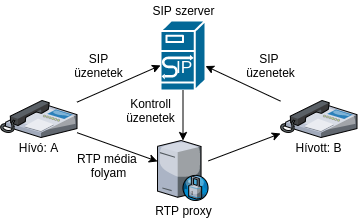
\includegraphics[width=0.5\textwidth, keepaspectratio]{figures/traditional_voip.png}
	\caption{Hagyományos VoIP hálózat}
	\label{fig:HVSpaces}
\end{figure}

Az ábrán egy általános hívásfelépítés látszik, ahol \textbf{A} hívja \textbf{B}-t. 
Ehhez, viszont SIP üzenetekben közölniük kell a SIP szerverrel, hogy ki milyen 
médiaformátumokat fogad el, melyik porton szeretnének kommunikálni a másikkal és 
hasonló információkat. A későbbiekben az összes ilyen protokoll kifejtésre fog
kerülni, hogy könnyebben látható legyen melyikre miért van szükség. Ha a SIP szerver
az összes üzenetet megkapta ahhoz, hogy létre tudjon hozni egy hívást, akkor az 
RTP proxynak megmondja, hogy hozzon létre egy hívást. Ha sikeresen létrejött a 
hívás, akkor kinyit két-két portot a hívásban résztvevő feleknek, amikre érkezhet
az adatfolyam. Azért nyit ki kettő portot kliensenként, mert az egyiken RTP 
csomagokat fog kezelni, míg a másikon RTCP (Real-time Transport Control Protocol) 
csomagokat. Mindezek mellett képes formátum konverziót is végrehajtani. Így ha 
a hívásban lévő két fél nem rendelkezik közös kódolási technikával, akkor is tudnak 
beszélgetni, mert az RTP proxy átfordítja mindkét félnek olyan kódolásra, amit 
képesek használni.

Ezzel a felépítéssel az a probléma, hogy az RTP proxy nem tud végtelen mennyiségű
hívást kezelni port hiányában vagy erőforrás hiány miatt. Így muszáj több példányt
telepíteni a hálózatba, ami jelentősen megbonyolítja a rendszer 
karbantarthatóságát és új problémákat idéz elő. Problémák, amiket ki szeretnék 
küszöbölni a munkám során:

\begin{itemize}
	\item \textbf{Skálázhatóság}: A fő kérdés az, hogy mire történjen a skálázás. 
	\begin{itemize}
		\item Ha nagyon sok a hívás, amik nem igényelnek nagy erőforrást, akkor
		kifuthat az RTP proxy a rendelkezésre álló portokból.
		\item Ha túl sok transzkódolást kell használni, akkor könnyen elfogyhatnak
		a rendelkezésre álló hardveres erőforrások.
		\item A skálázásnak ezenfelül automatikusan kellene működnie. 
	\end{itemize}
	\item \textbf{Rugalmasság}: Mi történik, akkor, ha az egyik RTP proxy szerver
	valamilyen oknál fogva nem üzemel tovább? Ilyenkor is valahogyan kezelni 
	kell a meglévő hívásokat és újakat is kell tudni létrehozni. Erre már van 
	megoldás, ahol egy Redis adatbázissal összetudjuk kötni a példányainkat. 
	Viszont ennek jelenleg van egy olyan hátránya, hogy csak manuálisan lehet 
	új példányt hozzácsatolni ehhez az adatbázishoz, ami rengeteg plusz munkát 
	jelent a nem elhanyagolható mértékű hibázási lehetőség mellett.
	\item \textbf{Automatizálás}: Hogyan lehet a lehető legkevesebb 
	karbantartással üzemeltetni egy ilyen rendszert? 
\end{itemize}

Amit szeretnék elérni, hogy az RTP proxy képes legyen Kubernetes rendszer alatt 
működni. Így megoldható lenne a fentebb említett problémák nagy része. De 
ehhez szükséges használni egy olyan szolgáltatáshálót, mint az L7mp. Ugyanis 
valahogyan kezelni kell a folyamatos UDP (User Datagram Protocol) forgalmat, amire
a jelenlegi szolgáltatáshálók közül kevesen képesek.

Ezenfelül kell egy kontroller, ami képes lesz hidat képezni az L7mp és az RTP 
proxy között. Erre azért van szükség, mert az L7mp nem képes automatikusan 
létrehozni a megfelelő forgalmi szabályokat. Ilyen szabályok szükségesek ahhoz, 
hogy egy hívás alatt a forgalom mindig ugyanahhoz az RTP proxyhoz érkezzen és 
ne összevissza a többi példány között.  

\section{Szakdolgozat felépítése}

Elsőnek a rendszerben résztvevő elemeket fogom részletesen bemutatni, hogy 
tágabb rálátást lehessen nyerni ezekre a technológiákra. Majd részletesebben 
foglalkozok azzal, hogy a hagyományos rendszer alatt hogyan működik egy hívás 
kezelése. Erre azért van szükség, mert az új rendszerben is pontosan ugyanígy fog 
működni, viszont az RTP proxy már nem csak egy egyszerű szerver lesz. 
Ezután a felépített rendszerről lesz részletesebben információ és arról, hogy a
kontroller hogyan működik ebben az egész megvalósításban. Amihez a használt
klienst is befogom mutatni, mert azzal közvetlen lehet kommunikálni az RTP proxyval
és tetszőleges számú hívás indítható el párhuzamosan. Végezetül pedig 
a tesztek értékelése lesz és összehasonlítása az új és a régi rendszer között. 